% =====================================================================
%  CLD 411 BTP Mid Semester Report -- Uday Pratap Singh (2023CH11201)
%
%  This file is written for the department's Overleaf template. Copy it into
%  the template project (the one that provides \logo, \participants,
%  \buildcover, \toc and jfm.bst), together with:
%      bibliography.bib      -> replaces the template's bibliography.bib
%      images/*.png          -> the figures of this report
%  Keep the template's own logos/ folder and style files untouched.
%
%  Every number here comes from the result files of the project repository:
%  https://github.com/uday338/adib-substrate-screening
% =====================================================================
\documentclass{report}
\usepackage{float}
\usepackage{graphicx}
\usepackage{natbib}
\usepackage{csquotes}

% ---- added for this report (all standard, all available on Overleaf) -------
\usepackage{amsmath,amssymb}
\usepackage{booktabs}
\usepackage{tabularx}
\usepackage{array}
\usepackage[version=4]{mhchem}   % \ce{...} for chemical formulae
\usepackage{enumitem}
% ---------------------------------------------------------------------------

\graphicspath{{images/}}
\newcolumntype{Y}{>{\raggedright\arraybackslash}X}

\newcommand{\phiox}{\varphi_{\mathrm{ox}}}
\newcommand{\phired}{\varphi_{\mathrm{red}}}
\newcommand{\phichl}{\varphi_{\mathrm{chlor}}}
\newcommand{\Ehull}{E_{\mathrm{hull}}}
\newcommand{\supervisor}{Prof.\ Anil Verma}
\newcommand{\studentname}{Uday Pratap Singh}
\newcommand{\entryno}{2023CH11201}

\title{CLD 411 BTP Mid Semester Report}
\bibliographystyle{jfm.bst}

\begin{document}

\logo{logos/IITD_Logo_Big.jpg}
\topic{Physics-Informed Computational Screening of Substrates for Aluminium Deposition in Anode-Free Aluminium Dual-Ion Batteries}
\ttitle{CLD 411 BTP Mid Semester Report}
\subject{Indian Institute of Technology Delhi}

\participants{
    \studentinfo{Uday Pratap Singh}{2023CH11201}{Chemical Engg.}{ch1231201@gmail.com}

    {Under supervision of \supervisor}

}

\buildmargins % display margins
\buildcover   % create the front cover of the document

\begin{abstract}
\noindent In an anode-free aluminium dual-ion battery (ADIB) aluminium is electroplated from a Lewis-acidic chloroaluminate melt onto a bare current collector. Aluminium is not being replaced as the plated species, which the electrolyte chemistry fixes; what the anode-free design replaces is the inactive aluminium foil, and the substrate that takes its place is what we screen. This report presents a reproducible, physics-informed screening framework for that substrate. Using Materials Project (MP) data for 830 entries in 67 chemical systems (metals, graphite, transition-metal nitrides, carbides, borides, silicides and aluminides), we apply pre-registered hard filters for thermodynamic stability and metallicity. We then compute, from grand-potential phase diagrams open to Al and Cl, each substrate's anodic limit in the melt and its reactivity towards deposited Al. Against verified literature measurements the computed anodic limit behaves as a thermodynamic lower bound: there are no contradictions, but materials protected by passive films or slow kinetics (TiN, Cr$_2$N, Ti) are under-rated. No stable metallic composition is both anodically stable to 1\,V and inert to Al at the plating potential. The resulting Pareto ranking gives 22 high-priority compositions, 18 of which also clear the lowest anodic scenario used for reporting, together with 19 medium-priority candidates; transition-metal borides are the most consistent family. The ranking uses DFT energies alone. A separate, leakage-controlled machine-learning (ML) benchmark on 1,566 MP entries tests whether the screen could later be extended to compositions that have no MP entry: composition-only models generalise to unseen chemical systems ($R^2 = 0.93 \pm 0.02$) but much less to unseen elements ($R^2 = 0.63 \pm 0.10$), and their uncertainty estimates do not yet track error, so that extension is not yet justified. These are preliminary computational results, not a discovery; surface and kinetic descriptors are planned for the second half of the semester.
\end{abstract}
\pagebreak

\section*{Acknowledgements}
\noindent I am grateful to my supervisor, \supervisor, for letting me take up this problem and for the direction he gave it. The scope of this project changed more than once in its early weeks, and his questions are what kept it pointed at a real electrochemical problem rather than at a convenient computational one. I am thankful for the time he gave to those discussions.

\noindent I would also like to thank the Materials Project team, whose open database and API this work depends on entirely, and the developers of pymatgen, matminer, scikit-learn and XGBoost, whose open-source tools made a screening study of this size possible on a laptop within a semester.

\vspace{1.0cm}
\begin{flushright}
\studentname,\\
\entryno
\end{flushright}
\pagebreak

\toc % creates the table of contents

%------------ Report body ----------------

\section{Introduction}

\subsection{The aluminium dual-ion battery}
Aluminium is abundant, and its three-electron redox chemistry makes it attractive for low-cost stationary storage. In the chloroaluminate aluminium--graphite dual-ion battery both electrodes draw on the electrolyte~\citep{Kravchyk2020b,Kravchyk2020}. On charge:
\begin{align}
\text{negative electrode:}\quad & \ce{4 Al2Cl7- + 3 e- -> Al + 7 AlCl4-} \label{eq:neg}\\
\text{positive electrode:}\quad & \ce{C_n + AlCl4- -> C_n[AlCl4] + e-} \label{eq:pos}
\end{align}
The electrolyte is an ionic liquid of \ce{AlCl3} and 1-ethyl-3-methylimidazolium chloride ([EMIm]Cl). Only a Lewis-acidic melt, with \ce{AlCl3} in excess over [EMIm]Cl, contains \ce{Al2Cl7-}, the species that is reduced to Al~\citep{Kravchyk2020b}. The melt contains no free \ce{Al^{3+}}, only \ce{AlCl4-} and \ce{Al2Cl7-}, so aluminium is the only metal that this electrolyte can deposit. That is why the plated species is fixed, and why the design freedom lies elsewhere.

\subsection{Why the substrate matters in an anode-free cell}
In an \emph{anode-free} cell there is no aluminium foil at the negative electrode. Al is plated during the first charge onto a bare current collector (the substrate) and stripped from it on discharge~\citep{WangL2021}. Two reasons motivate removing the foil. First, the capacity of these cells is set by the \ce{Al2Cl7-} content of the anolyte rather than by the anode, and the low charge-storage capacity of the anolyte is what limits the technology~\citep{Kravchyk2020}; a thick foil therefore adds mass and volume without adding capacity. Second, the foil is not inert in service: reviewing the work of Tak and co-workers, Kravchyk and Kovalenko report that ``Al surface corrodes in chloroaluminate melts'' and that ``the corrosion enhances significantly upon increasing their acidity''~\citep{Kravchyk2020b}. We do not quantify the energy-density gain here, because none of the sources in our literature table measures one.

Equation~\eqref{eq:neg} fixes the plated species: replacing aluminium would mean a different battery. What is replaced is the foil, and the substrate that takes its place must do a harder job, facing three problems at once:
\begin{enumerate}[leftmargin=*]
\item \textbf{Attack by the melt.} After all Al is stripped, the bare collector sits at potentials positive of Al. Many metals are oxidised (chlorinated) by chloroaluminate melts in this range~\citep{Wang2018,Oh2018,Reed2013}.
\item \textbf{Alloying with the deposited Al.} Al can form intermetallics with the substrate and consume Al irreversibly. For example, Al underpotential deposition on V gives \ce{Al3V} and \ce{AlV3}~\citep{Cvetkovic2021}.
\item \textbf{Nucleation and morphology.} Deposit morphology and reversibility depend on metal--substrate bonding~\citep{Zheng2021}.
\end{enumerate}
The first two problems can be computed from bulk thermodynamics; the third needs surface calculations and is planned for the second half of the semester (Section~\ref{sec:plan}).

\subsection{Motivation for this work}
A materials choice of this kind is usually made by testing a handful of candidates in the laboratory. That is slow, and it explores only the materials someone already suspected. The alternative is to compute the two bulk requirements above for every plausible material at once, using data that already exist, and to let the shortlist come out of explicit physical criteria rather than intuition. The Materials Project~\citep{Jain2013} holds density-functional-theory energies for tens of thousands of inorganic compounds, which is enough to ask whether a substrate can survive the melt, and whether it will react with the aluminium plated onto it.

What such a screen cannot do is decide by itself which criteria matter, or how far to trust the numbers. The motivation of this work is therefore as much methodological as chemical: to build a screen whose every threshold has a stated source, which is tested against measurements that already exist, and which reports its own failures. Machine learning enters only where there are enough data to test it honestly, and is kept out of the ranking.

\subsection{Research question and objectives}
\noindent\textbf{Research question.} \emph{Which conductive materials can serve as substrates for stable and reversible Al deposition in chloroaluminate ADIBs, and what computable descriptors separate them?}

\noindent Experimental substrate data are far too sparse for supervised machine learning: about a dozen materials, measured under differing conditions. The project is therefore framed as \textbf{physics-informed screening}, not black-box prediction of battery performance. Objectives for the mid-semester stage:
\begin{enumerate}[leftmargin=*,itemsep=2pt]
\item Build a reproducible pipeline on real Materials Project data~\citep{Jain2013}.
\item Define physically justified descriptors and hard filters, with every threshold fixed and sourced \emph{before} any result is seen.
\item Benchmark classical ML models (Ridge, random forest, XGBoost) with leakage-controlled, grouped validation, to establish whether the screen can later be extended to materials that have no DFT data.
\item Validate the framework against verified literature, reporting disagreement rather than tuning it away.
\item Produce a preliminary shortlist of candidates for DFT or experimental validation later in the year.
\end{enumerate}

\noindent Throughout, three kinds of knowledge are kept separate: \textbf{(A) computed} (MP data, or quantities derived deterministically from MP energies), \textbf{(B) literature} (verified experimental observations) and \textbf{(C) inferred} (ML predictions and screening conclusions).

% =====================================================================
\pagebreak
\section{Literature Review}
\label{sec:lit}

Table~\ref{tab:lit} summarises the literature observations used in this work. Each was verified word for word against the open-access full text or the published abstract; the evidence text, conditions and verification level for every row are recorded in the project's literature table (\texttt{data/literature\_benchmark.csv}, 24 rows: 12 verified from full text, 5 from abstracts, 2 accessible only as summaries and 5 labels carried over from earlier project notes for which no source could be found).

\begin{table}[H]
\centering
\caption{Verified literature on substrates and current collectors in chloroaluminate electrolytes. ``Positive'' = tested as a positive (cathode) current collector.}
\label{tab:lit}
\small
\begin{tabularx}{\textwidth}{@{}p{3.3cm} p{1.8cm} p{2.9cm} Y@{}}
\toprule
Source & Electrode side & Electrolyte & Verified observation \\
\midrule
Wang \emph{et al.} 2018~\citep{Wang2018} & positive & \ce{AlCl3}:[EMIM]Cl $=2$ & Oxidation onsets 0.62 (Cr), 0.92 (stainless steel), 1.0 (Al), 1.1\,V (Ti) vs Al; Au etched at 2\,V; Au and Pt unstable above 2\,V; TiN and \ce{Cr2N} stable until electrolyte oxidation at 2.5--3\,V; TiN more stable than W, Mo and glassy carbon \\
Oh \emph{et al.} 2018~\citep{Oh2018} & positive & acidic \ce{AlCl3}--[EMIm]Cl & Ni electrochemically and chemically unstable in an expanded window; Mo stable \\
Shi \emph{et al.} 2019~\citep{Shi2019}; Reed \& Menke 2013~\citep{Reed2013} & positive & 1.3:1 & Most metals corrode; stainless-steel corrosion current can be mistaken for battery capacity \\
Cvetkovi\'c \emph{et al.} 2021~\citep{Cvetkovic2021} & negative & \ce{AlCl3}--NaCl, 200\,\textdegree C & Al underpotential deposition on V forms \ce{Al3V} and \ce{AlV3} \\
Kravchyk \emph{et al.} 2020~\citep{Kravchyk2020} & negative & \ce{AlCl3}--EMIMCl & Al electroplating on a metallic Al collector in Al--graphite dual-ion batteries \\
Kravchyk \& Kovalenko 2020~\citep{Kravchyk2020b} (review of Tak and co-workers) & negative & acidic chloroaluminate RTIL & ``Al surface corrodes in chloroaluminate melts'', and the corrosion increases with acidity; most metallic current collectors are incompatible with these electrolytes \\
\bottomrule
\end{tabularx}
\end{table}

Two further sources are cited for context but \emph{not} used as ground truth, because only a summary was accessible: Zheng \emph{et al.}~\citep{Zheng2021} (oxygen-mediated Al--substrate bonding, reported reversibility 99.6--99.8\%) and Wang L.\ \emph{et al.}~\citep{WangL2021} (initial-anode-free Al batteries with various anodic collectors).

\paragraph{Research gap.} Current-collector studies in the ADIB literature concern almost exclusively the \textbf{positive} electrode, where the collector sits at about 2--2.5\,V vs Al. Our literature search (September 2026, limited to accessible abstracts and open full texts) found no systematic screen of \emph{negative-side} (anode-free) substrates across materials classes. We also found that several labels in the project's starting notes (``W, Mo, glassy carbon, TiN: stable'') come from positive-electrode tests. They describe resistance to oxidation at high potential, which is a different requirement from reversible Al plating near 0\,V, and are therefore recorded with their electrode side.

% =====================================================================
\pagebreak
\section{Methodology}
\label{sec:method}

\subsection{Framework overview}
The pipeline has six stages (Figure~\ref{fig:funnel}): (0) a candidate space with a stated rationale for each family; (1) MP retrieval, cached so the analysis runs offline; (F1) a thermodynamic-stability filter; (F2) a metallicity filter; (3) the substrate's stability window in the electrolyte; (4) Pareto ranking with sensitivity analysis; and (5) validation against the literature. Every threshold and every validation rule was written down, with its source, before any descriptor was computed or compared (project file \texttt{docs/descriptors.md}).

\subsection{Candidate space and data}
The screening space contains 67 chemical systems in six families, each included for a stated reason:
\begin{itemize}[leftmargin=*,itemsep=1pt]
\item \textbf{elemental metals and graphite} (19): conventional collectors and every single-element literature reference; graphite is the closest MP stand-in for graphite paper and glassy carbon;
\item \textbf{transition-metal nitrides} (9): metallic, and TiN and \ce{Cr2N} are measured stable positive collectors~\citep{Wang2018};
\item \textbf{carbides, borides and silicides} (9 each): metallic refractory compounds, chemically analogous to the nitrides (hypothesis);
\item \textbf{transition-metal aluminides} (12): pre-aluminised substrates that cannot alloy further (hypothesis, motivated by~\citep{Cvetkovic2021}).
\end{itemize}
MP gives 830 entries (330 unique compositions) in this space. Oxides, sulfides and phosphides appear only in the ML training set (Section~\ref{sec:ml}): they were added there to give grouped validation enough chemical systems, not because they are substrate candidates. Stainless steel (an alloy) and glassy carbon (amorphous) have no single MP entry and are treated as literature-only references.

\subsection{Hard filters}
\textbf{F1, thermodynamic stability.} Keep entries whose energy above the convex hull, $\Ehull$, is at most the 90th percentile of the metastability of experimentally observed crystals: 67\,meV/atom in general and 195\,meV/atom for nitrides~\citep{Sun2016}. $\Ehull$ is used only as a filter, never as an ML feature (Section~\ref{sec:ml}).

\noindent\textbf{F2, conduction proxy.} Keep entries that are metallic in PBE (band gap $=0$). A current collector must conduct electrons. PBE underestimates band gaps, and metallic character is not the same as high conductivity; these caveats are carried into the limitations.

\subsection{Stability window of a substrate in the melt}
\label{sec:window}
The melt is treated as a reservoir of Al and Cl tied together through \ce{AlCl3}. At electrode potential $\varphi$ (V vs Al/\ce{AlCl3}) the chemical potentials are
\begin{equation}
\mu_{\mathrm{Al}}(\varphi) = \mu^{\circ}_{\mathrm{Al}} - 3e\varphi, \qquad
\mu_{\mathrm{Cl}}(\varphi) = \tfrac{1}{3}\left[g(\ce{AlCl3}) - \mu_{\mathrm{Al}}(\varphi)\right],
\label{eq:mu}
\end{equation}
where $\mu^{\circ}_{\mathrm{Al}}$ is the energy per atom of Al metal and $g(\ce{AlCl3})$ the hull energy of \ce{AlCl3}, both taken from the same MP entry set. For every substrate composition we build, on a 0.01\,V grid, the grand-potential phase diagram open to Al and Cl, using every MP entry in the \{substrate, Al, Cl\} space (pymatgen~\citep{Ong2013}). The driving force for reaction with the reservoir is
\begin{equation}
r(\varphi) = \frac{\Omega_{\mathrm{hull}}(\varphi) - \Omega_{\mathrm{closed}}(\varphi)}{N_{\mathrm{substrate}}} \le 0 ,
\end{equation}
and the equilibrium products classify the reaction: products gaining Cl indicate \emph{chlorination}, products losing Al indicate \emph{Al extraction} (dealloying), and products gaining Al indicate \emph{alloying}. Three descriptors follow:
\begin{itemize}[leftmargin=*,itemsep=1pt]
\item $\phiox$, the \textbf{anodic limit}: the onset of the first anodic reaction (chlorination or Al extraction). For a plain metal M it is equivalent to $\mathrm{M} + \tfrac{n}{3}\,\mathrm{AlCl_3} \rightarrow \mathrm{MCl}_n + \tfrac{n}{3}\,\mathrm{Al}$ with $E = \Delta G/(ne)$;
\item $\phired$: the highest potential at which the substrate still takes up Al (alloying);
\item $r_0 = r(0)$: the driving force for reaction with Al metal at the plating potential.
\end{itemize}
A composition is called \textbf{inert to Al} when $|r_0| < 1$\,meV/atom, the tolerance used when the phase diagram is constructed; that is, no exchange with the reservoir lowers its energy at 0\,V. Otherwise $r_0$ is negative and its magnitude is quoted, since the distinction between, say, $-0.02$ and $-1.6$\,eV/atom matters far more than a label. This threshold is used identically in the tables and in the discussion.
$\phiox$ is a \textbf{thermodynamic lower bound}. Below it corrosion is impossible, but a material may survive above it through passivation or slow kinetics. The model neglects the activity of \ce{AlCl3} in an acidic melt, dissolution and complexation of chloride products (which \emph{lowers} the real onset), gas entropy, temperature (DFT energies are at 0\,K), kinetics and passive films.

MP mixes GGA/GGA+$U$ and r$^2$SCAN energies in two ways: consistently over each requested chemical space (client-side), or per material (server-side). Chloride formation energies differ between the two (\ce{AlCl3}: $-1.69$ vs $-1.97$\,eV/atom). We therefore compute $\phiox$ with both and report the spread as a \emph{method uncertainty}.

\subsection{Ranking and sensitivity}
Compositions passing F1 and F2 (each represented by its lowest-$\Ehull$ metallic polymorph) are ranked by non-dominated sorting (Pareto layers) on three objectives, with no weights: maximise $\phiox$, maximise $r_0$ (least reactive with Al) and minimise $\Ehull$. Layers 1--2 are ``high priority'', 3--4 ``medium'', the rest ``low''. The potential that a negative collector reaches after complete stripping depends on the cell's discharge cut-off, so no single anodic threshold is imposed. Survivors are reported for cut-offs of 0.5, 1.0, 1.5 and 2.0\,V, and for $0.5\times$, $1\times$ and $1.5\times$ the F1 window. A candidate's confidence is ``higher'' when its tier is the same under both MP energy routes and the phase is experimentally known (ICSD).

\subsection{Machine-learning benchmark}
\label{sec:ml}

\textbf{What the ML is for, and what it is not.} The shortlist in this report is built entirely from MP DFT energies and the grand-potential phase diagrams of Section~\ref{sec:window}. No ML model enters the filters, the descriptors or the ranking: for a material that already has an MP entry, the DFT value is known, and predicting it again would add nothing. The ML benchmark is instead a feasibility test for the next stage, where we want to screen compositions that have \emph{no} MP entry, such as the hypothetical ternary borides and nitrides in the plan of Section~\ref{sec:plan}. Only a composition-only model can do that, so the question is whether such a model can be trusted outside the chemistry it was trained on. The results in Section~\ref{sec:mlres} answer it: yes for an unseen chemical system, not yet for an unseen element, and not at all at the level of individual predictions, because no uncertainty estimate we tested tracks the error. Until that is fixed, candidates proposed by ML cannot be ranked alongside candidates with DFT data.

\noindent\textbf{Target and data.} The target is the MP formation energy per atom, a benchmark with full coverage and not the screening criterion. For materials already in MP the DFT value is used directly. The dataset holds 1,653 entries in 76 chemical systems (elements, nitrides, carbides, borides, oxides, silicides, phosphides and sulfides). Entries more than 1\,eV/atom above the hull (87) were removed by a cut-off fixed in advance, leaving 1,566.

\noindent\textbf{Features.} 132 Magpie elemental-property statistics~\citep{Ward2016} computed with matminer~\citep{Ward2018} (127 non-constant), plus the number of elements: the \emph{composition-only} set. A \emph{full} set adds density, volume per atom, band gap and number of sites. These need a relaxed DFT structure, so the full set is circular for genuinely new materials.

\noindent\textbf{Leakage audit.} Before any model is fitted, each column is checked for (i) identity with the target, which halts the run; (ii) grouped $R^2$ from that column alone; and (iii) constancy within a chemical system. $\Ehull$ is excluded because for elemental entries it equals the formation energy exactly.

\noindent\textbf{Models and validation.} Ridge (regularisation strength chosen by grouped CV inside each training fold), random forest~\citep{Pedregosa2011} and XGBoost~\citep{Chen2016}. Three splits are used: shuffled 5-fold KFold; \textbf{leave-one-chemical-system-out} (76 folds; the headline); and \textbf{leave-one-element-out} (23 folds; every system containing the element is held out). Leave-one-system-out holds out, for example, N--Ti while Ti and C--Ti remain in training, so it tests an unseen \emph{system}, not an unseen \emph{element}; hence the third split.

\noindent\textbf{Scoring.} Metrics are computed on pooled out-of-fold predictions and also \emph{system-balanced}: each of the 76 systems counts equally, because oxides are 44\% of the rows. Standard errors come from 1,000 bootstrap resamples of whole chemical systems, shared across models and splits so that differences get paired SEs. Per-fold $R^2$ is not averaged: a single held-out system can span only $\sim$0.01\,eV/atom, which makes its $R^2$ meaningless. Feature importance is permutation importance on held-out chemical systems.

\noindent\textbf{External test.} Transition-metal aluminides are absent from the training set, so their MP formation energies test the models on an unseen family. The applicability domain is measured as the mean distance to the five nearest training compositions from \emph{other} chemical systems, in standardised Magpie space.

% =====================================================================
\pagebreak
\section{Description of Software and Computational Procedure}
\label{sec:setup}

\subsection{Data sources}
All materials data come from the Materials Project~\citep{Jain2013}, retrieved through its API (\texttt{mp-api} 0.46.5) in September 2026. Three kinds of query are used: summary records for the 830 entries of the screening space; the full set of entries in each \{substrate, Al, Cl\} chemical space, used to build the phase diagrams; and the server-side thermodynamic records for the same spaces, used as the independent second energy route. Every download is cached on disk, so the whole analysis reruns offline and gives identical numbers. The literature table is maintained by hand as a separate file, with the evidence text and a verification level for each row.

\subsection{Software}
The phase diagrams, chemical potentials and grand-potential constructions use pymatgen~\citep{Ong2013} (version 2026.5.4). Composition features are the Magpie set~\citep{Ward2016} as implemented in matminer~\citep{Ward2018} (0.10.1). Models are Ridge and random forests from scikit-learn~\citep{Pedregosa2011} (1.9.0) and XGBoost~\citep{Chen2016} (3.4.1); figures use matplotlib. The pipeline is written in Python 3.14 as eight modules, one per stage, with a single script that runs them in order.

\subsection{Hardware and run times}
Everything runs on an ordinary laptop (8 CPU cores); no HPC allocation was needed at this stage. Building the stability windows for all 330 compositions by both energy routes takes about 20 minutes with six worker processes, and is cached afterwards. The full machine-learning benchmark, which refits three models over 76 leave-one-system-out folds, 23 leave-one-element-out folds and 5 random folds for two feature sets, and then computes permutation importances, takes about 1.5 hours. Rerunning everything else from the cache takes 35 seconds.

\subsection{Reproducibility}
\begin{verbatim}
python run_all.py --offline      # ~35 s; no network or API key needed
python run_all.py                # refetch MP data and refit the ML benchmark
\end{verbatim}
The random seed is fixed at 42 throughout. The Materials Project is a live database, so a later refetch may shift individual numbers; the cached copy used for this report is kept with the code. Table~\ref{tab:outputs} lists the files that hold the results quoted in Section~\ref{sec:results}.

\begin{table}[H]
\centering
\caption{Project files holding the results reported here.}
\label{tab:outputs}
\small
\begin{tabularx}{\textwidth}{@{}l Y@{}}
\toprule
File & Content\\
\midrule
\texttt{docs/descriptors.md} & pre-registered filters, thresholds and validation rules, with sources\\
\texttt{data/literature\_benchmark.csv} & 24 literature rows with DOI, conditions and verification level\\
\texttt{results/screening\_candidates.csv} & all 330 compositions with descriptors, status, tier and knowledge-type tags\\
\texttt{results/shortlist.csv} & high and medium candidates with reasons, and rejected examples\\
\texttt{results/validation.csv} & known-material validation verdicts\\
\texttt{results/model\_comparison.csv}, \texttt{leakage\_audit.csv} & ML benchmark and leakage audit\\
\texttt{adib\_workflow.ipynb} & executed notebook of the complete workflow\\
\bottomrule
\end{tabularx}
\end{table}

% =====================================================================
\pagebreak
\section{Results and Discussion}
\label{sec:results}

\subsection{ML benchmark on real data}
\label{sec:mlres}
The leakage audit of all 132 columns found 67 clean, 64 group proxies (constant within a system, mostly Magpie min/max/range statistics), and no feature identical to the target. $\Ehull$ was flagged (equal to the target on 8.9\% of rows) and is excluded. Table~\ref{tab:ml} and Figure~\ref{fig:ml} give the composition-only results.

\begin{table}[H]
\centering
\caption{Composition-only formation-energy models on 1,566 MP entries (76 chemical systems). $R^2 \pm$ group-bootstrap SE.}
\label{tab:ml}
\small
\begin{tabular}{@{}lccccc@{}}
\toprule
 & Random & \multicolumn{2}{c}{Leave-one-system-out} & \multicolumn{2}{c}{Leave-one-element-out}\\
\cmidrule(lr){3-4}\cmidrule(lr){5-6}
Model & 5-fold & pooled & balanced & pooled & balanced\\
\midrule
Ridge & $0.940\pm0.017$ & $0.870\pm0.027$ & $0.825\pm0.047$ & $0.747\pm0.035$ & $0.706\pm0.048$\\
Random forest & $0.966\pm0.010$ & $\mathbf{0.931\pm0.021}$ & $\mathbf{0.920\pm0.021}$ & $0.634\pm0.095$ & $0.741\pm0.040$\\
XGBoost & $0.966\pm0.010$ & $0.922\pm0.014$ & $0.920\pm0.020$ & $0.634\pm0.076$ & $0.748\pm0.035$\\
\bottomrule
\end{tabular}
\end{table}

\begin{figure}[H]
\centering
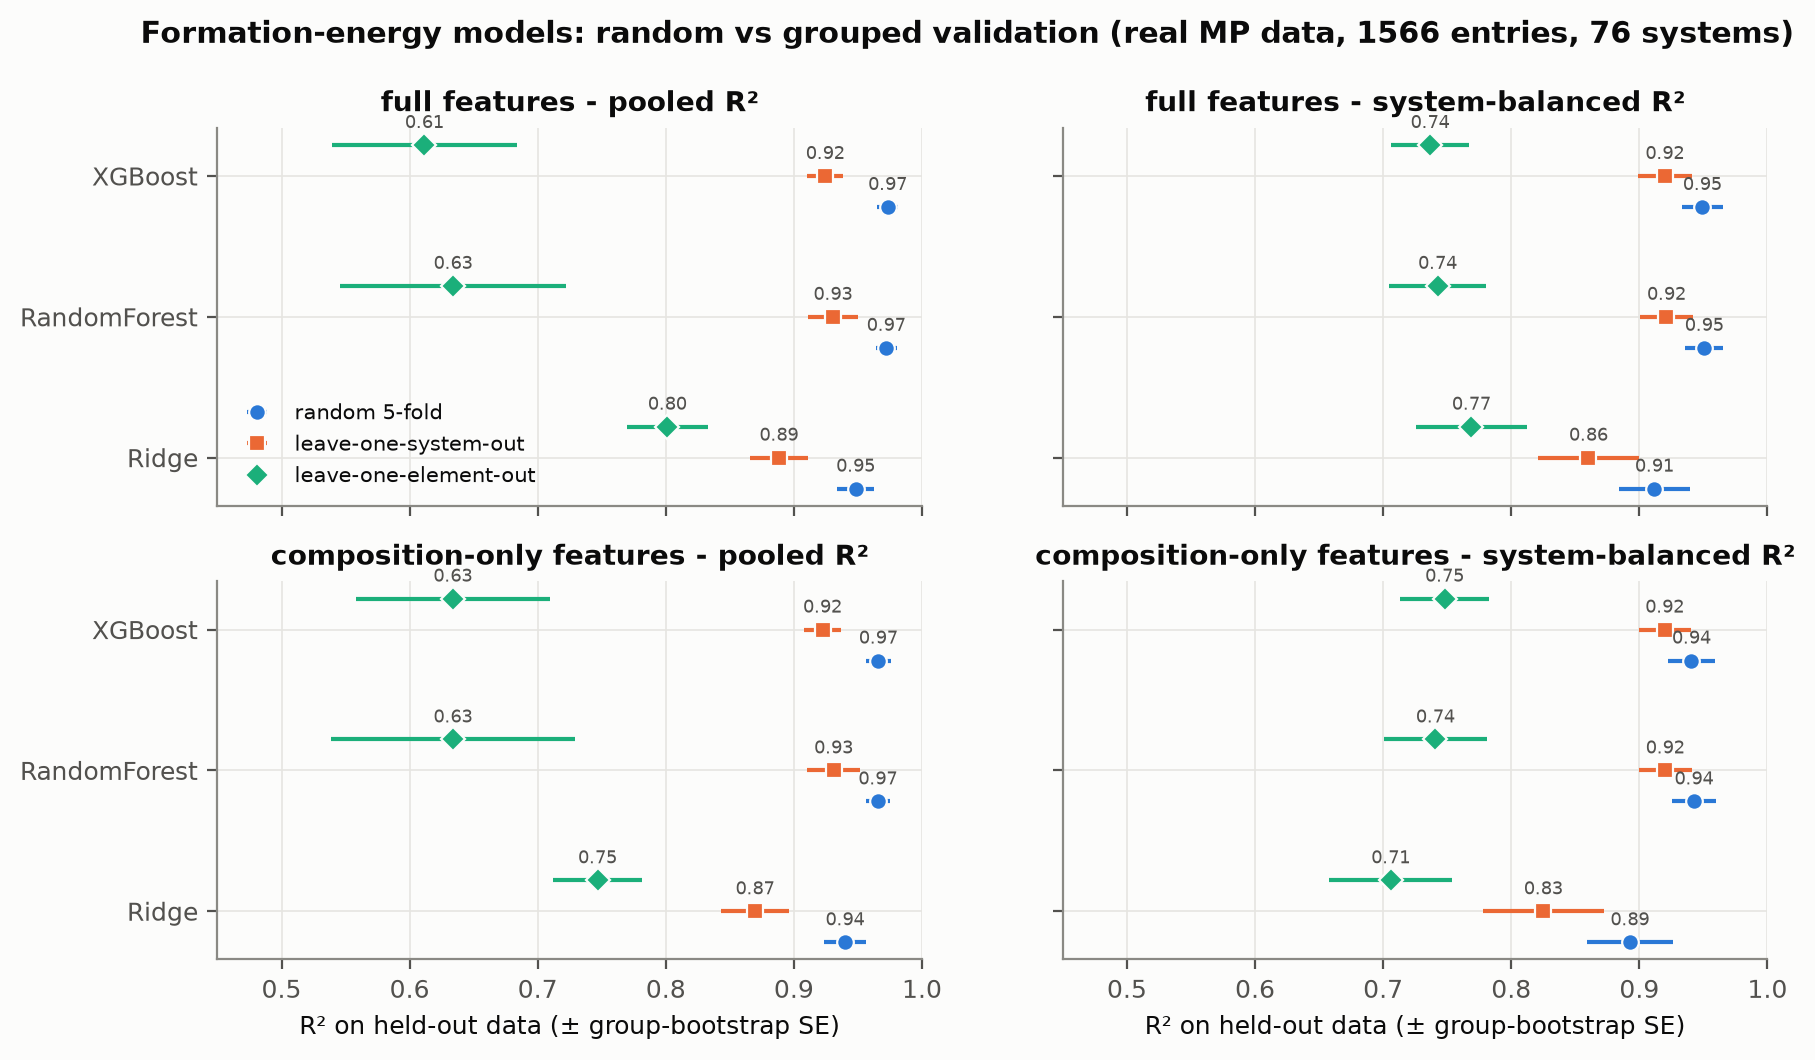
\includegraphics[width=\textwidth]{04_model_performance.png}
\caption{Held-out $R^2$ under random, leave-one-system-out and leave-one-element-out validation, pooled and system-balanced, for both feature sets.}
\label{fig:ml}
\end{figure}

\begin{itemize}[leftmargin=*,itemsep=2pt]
\item \textbf{Unseen chemical systems.} The random forest reaches $R^2 = 0.931 \pm 0.021$ (MAE $0.234$\,eV/atom). The random-to-grouped gap is $0.035 \pm 0.015$ pooled and $0.022 \pm 0.008$ balanced: modest, but larger than twice its SE (Figure~\ref{fig:gap}).
\item \textbf{Pooled and balanced agree} within 2\,SE (difference $0.011 \pm 0.019$), so the large oxide share does not distort the headline.
\item \textbf{Unseen elements are much harder.} The tree models fall to $R^2 \approx 0.63$ pooled. Ridge has the higher point estimate ($0.75$), but the SEs do not resolve the difference.
\item \textbf{DFT/structure features add nothing.} The full minus composition-only grouped $R^2$ is $-0.019$ (Ridge), $0.000$ (random forest) and $-0.002$ (XGBoost), so the set usable for new materials costs nothing.
\item \textbf{Permutation importance} (Figure~\ref{fig:imp}): the tree models rely on melting-temperature statistics, the range of Mendeleev number and the spread of unfilled valence shells; Ridge relies on elemental band-gap and electronegativity statistics. Collinear Magpie statistics share credit, so these should be read as families of descriptors, not single causes.
\end{itemize}

\begin{figure}[H]
\centering
\begin{subfigure}{0.49\textwidth}
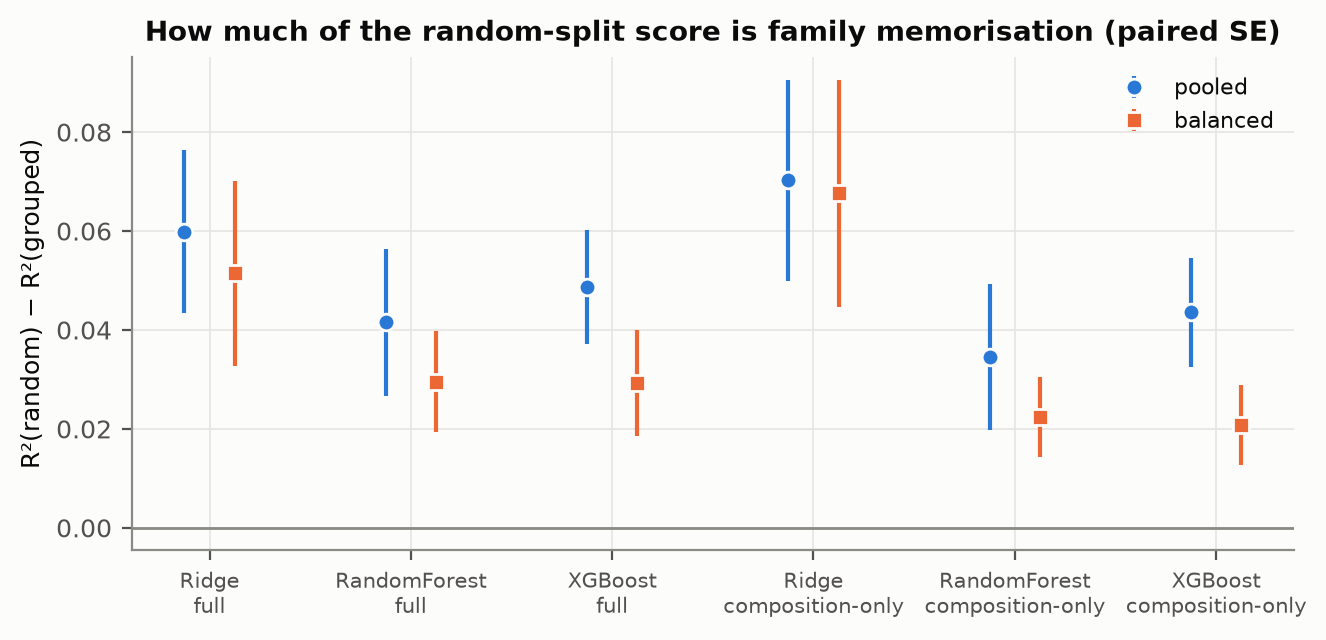
\includegraphics[width=\textwidth]{05_random_vs_grouped_gap.png}
\caption{Random-to-grouped $R^2$ gap (paired SE).}
\label{fig:gap}
\end{subfigure}\hfill
\begin{subfigure}{0.49\textwidth}
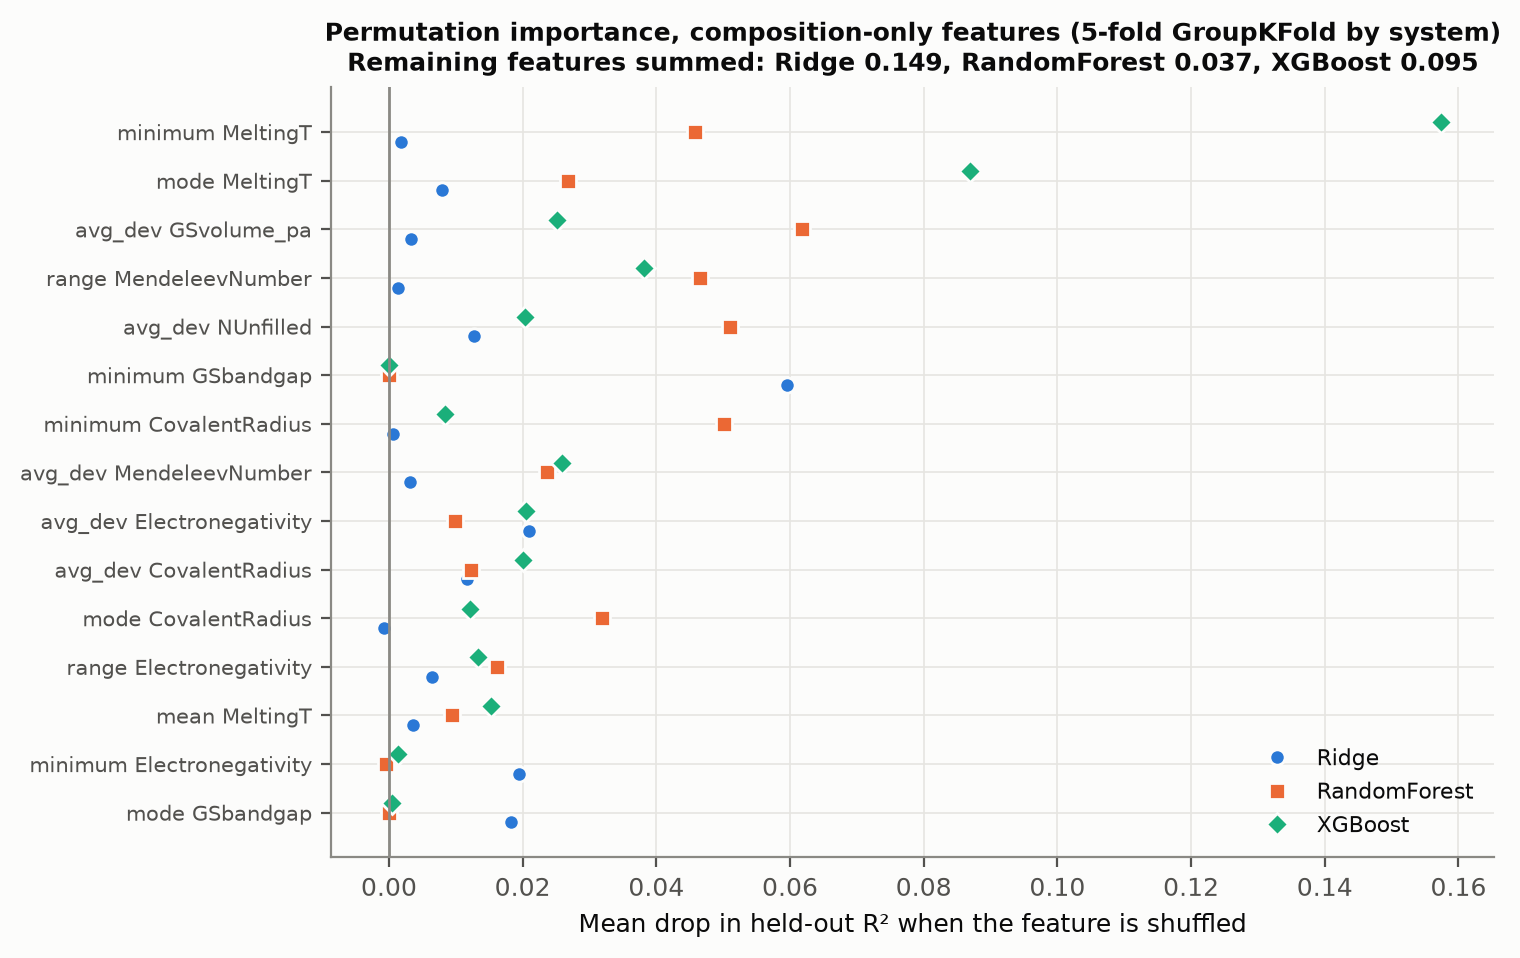
\includegraphics[width=\textwidth]{06_feature_importance.png}
\caption{Permutation importance, composition-only.}
\label{fig:imp}
\end{subfigure}
\caption{How much of the random-split score comes from memorising chemical families, and which features the models use.}
\end{figure}

\subsection{External test and applicability domain}
On the 128 aluminide entries, which come from a family never seen in training, the random forest has MAE $0.158$\,eV/atom (XGBoost $0.193$, Ridge $0.276$). However, neither distance to the training set (Spearman $\rho = -0.13$), nor random-forest tree spread ($\rho = 0.02$), nor disagreement between models ($\rho = 0.18$) predicts which predictions are wrong (Figure~\ref{fig:ad}). A usable uncertainty estimate is therefore a prerequisite before ML is applied to hypothetical compositions.

\begin{figure}[H]
\centering
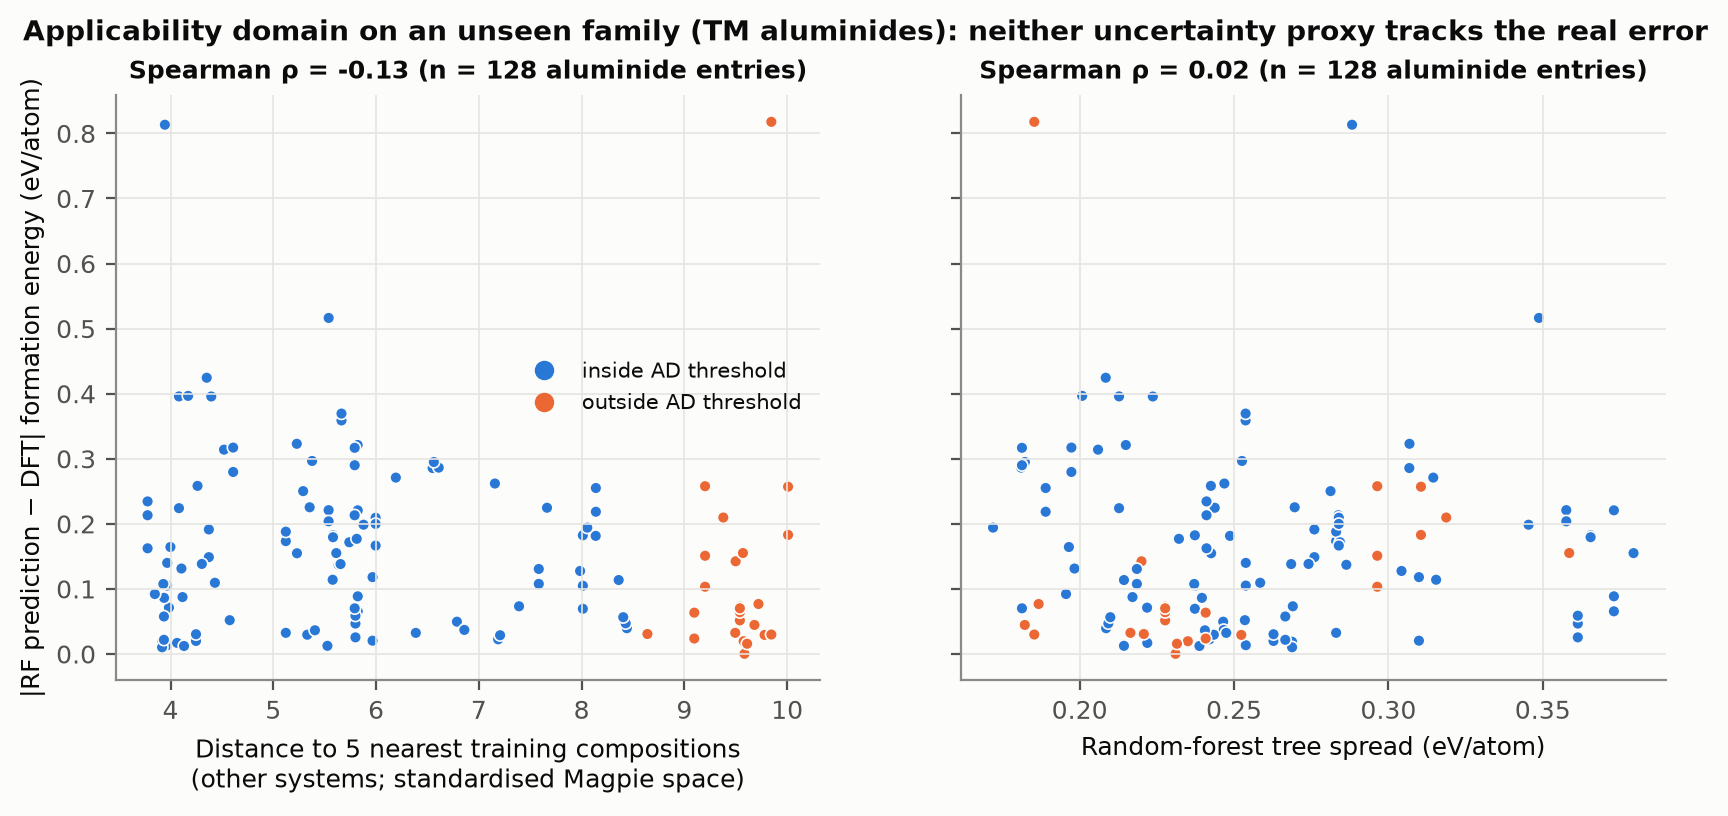
\includegraphics[width=0.95\textwidth]{11_applicability_domain.png}
\caption{Random-forest error on unseen aluminides against applicability-domain distance (left) and tree spread (right).}
\label{fig:ad}
\end{figure}

\subsection{Screening funnel}
Table~\ref{tab:funnel} and Figure~\ref{fig:funnel} show how many compositions survive each stage. \textbf{No composition is both anodically stable to 1\,V and inert to Al at the plating potential.} Almost every transition-metal substrate can alloy with the deposited Al (e.g.\ \ce{Al3Ni}, \ce{Al2Cu}, \ce{Al5W}, \ce{Al4C3}), and the few that cannot have anodic limits below 1\,V. This trade-off is why a Pareto ranking is used instead of a single score.

\begin{table}[H]
\centering
\caption{Screening funnel (thresholds fixed in advance).}
\label{tab:funnel}
\small
\begin{tabular}{@{}lr@{}}
\toprule
Stage & Count\\
\midrule
MP entries in the screening space & 830\\
Unique compositions & 330\\
Pass F1 ($\Ehull$ within the metastability window) & 254\\
Pass F1 and F2 (metallic) & 250\\
$\phiox \ge 0.5$\,V & 93\\
$\phiox \ge 1.0$\,V & 25\\
$\phiox \ge 1.0$\,V and stable against Al at 0\,V & \textbf{0}\\
High-priority tier (Pareto layers 1--2) & 22\\
High-priority tier and $\phiox \ge 0.5$\,V (the shortlist reported in Table~\ref{tab:short}) & 18\\
\bottomrule
\end{tabular}
\end{table}

\begin{figure}[H]
\centering
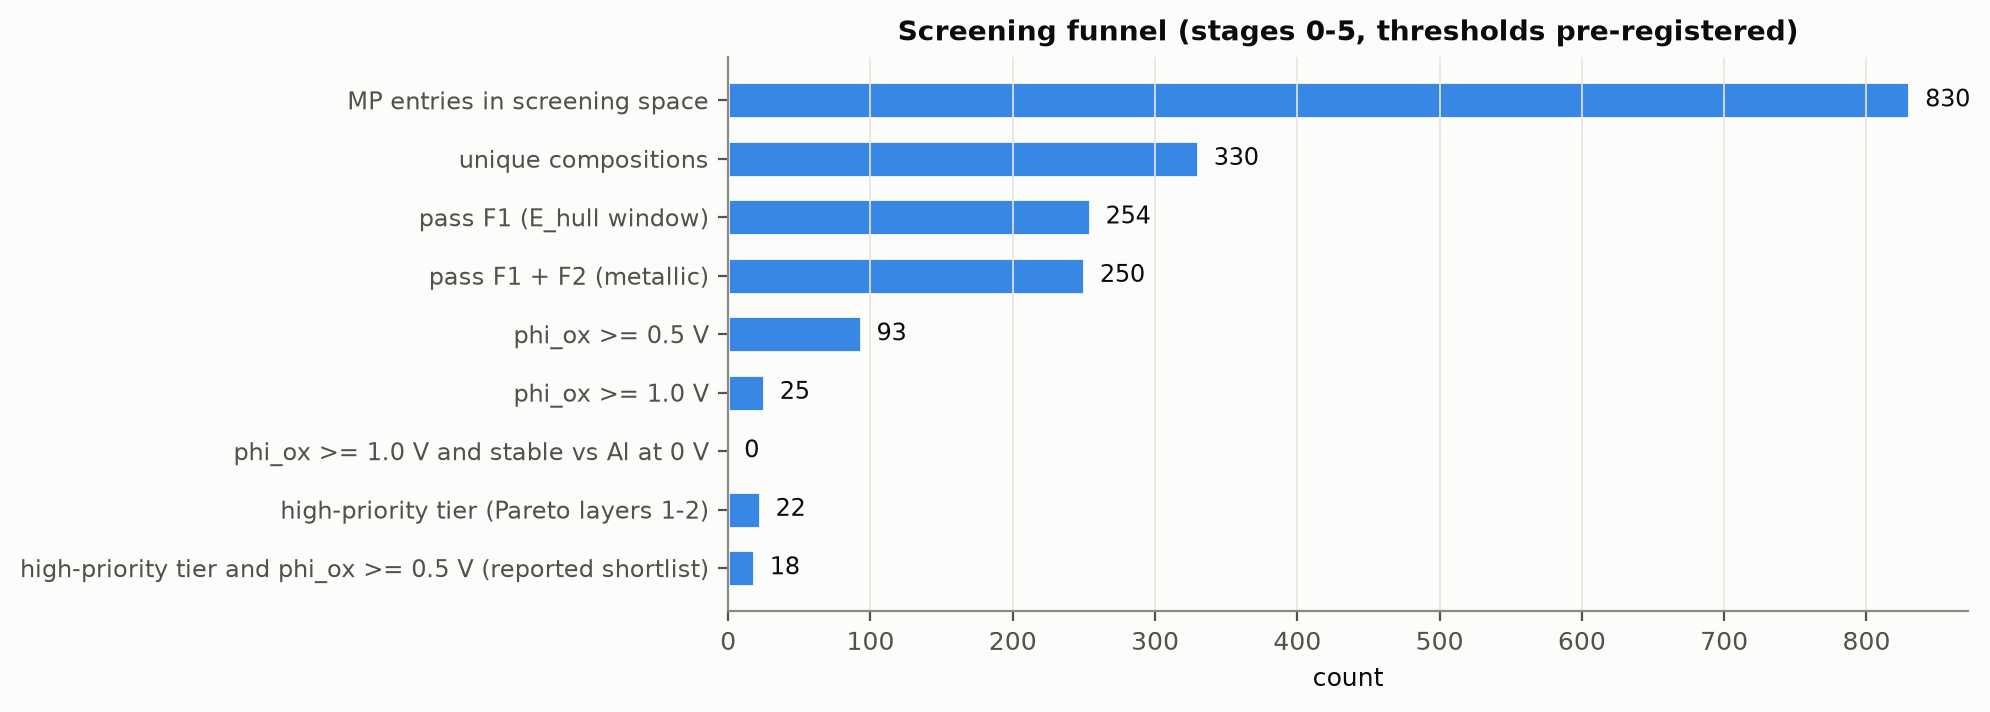
\includegraphics[width=0.85\textwidth]{07_screening_funnel.png}
\caption{Screening funnel. The Pareto ranking places 22 compositions in the high-priority tier; 18 of them also clear the lowest anodic scenario ($\phiox \ge 0.5$\,V) and are the ones reported in Table~\ref{tab:short}. The four excluded are Al-rich aluminides, from which Al is extracted at 0.01\,V.}
\label{fig:funnel}
\end{figure}

\noindent\textbf{Sensitivity.} The shortlist depends far more on the required anodic potential than on the stability window (Figure~\ref{fig:sens}). At the registered window the survivors number 249, 93, 25, 3 and 1 for cut-offs of 0, 0.5, 1.0, 1.5 and 2.0\,V. Above 1.5\,V only graphite, Au and Pt remain. The two MP energy routes give $\phiox$ values that differ by a median of 0.02\,V (90th percentile 0.16\,V, maximum 0.42\,V), and 88\% of candidates keep the same tier under both.

\begin{figure}[H]
\centering
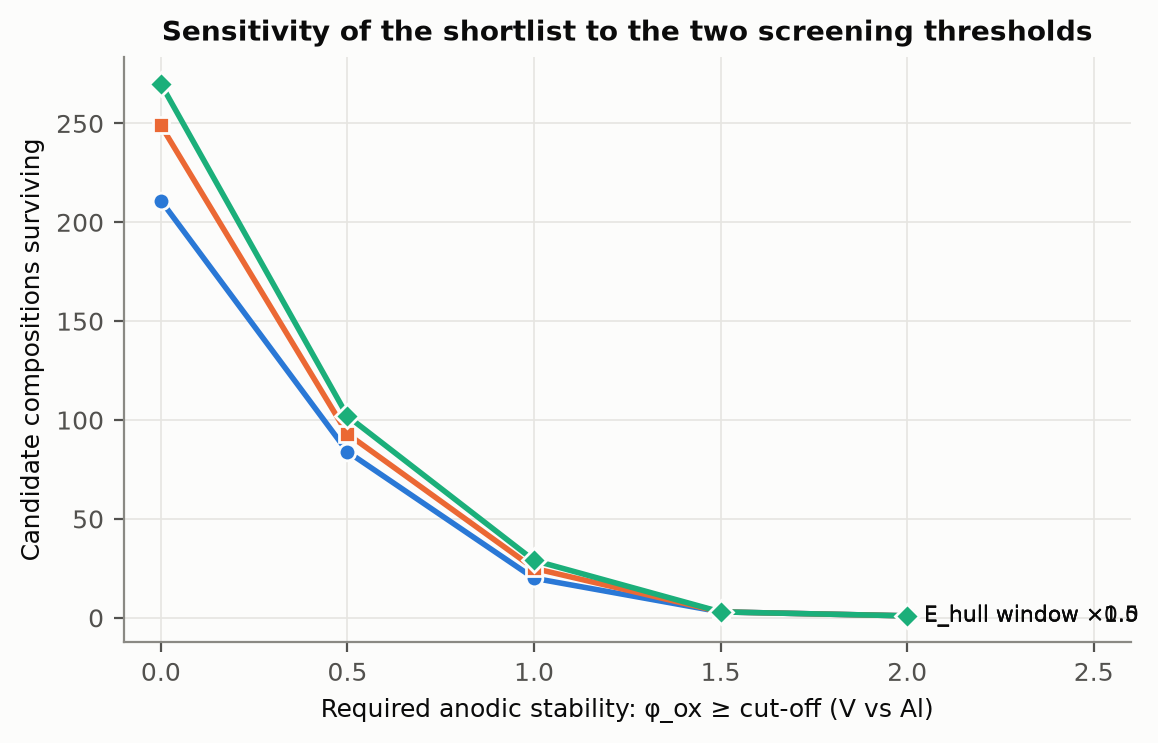
\includegraphics[width=0.62\textwidth]{12_sensitivity.png}
\caption{Candidates surviving as a function of the anodic cut-off and the $\Ehull$ window.}
\label{fig:sens}
\end{figure}

\subsection{Known-material validation}
\label{sec:val}
The validation rules were fixed before the comparison. The framework \emph{agrees} if the measured limit is at least $\phichl - 0.2$\,V and \emph{disagrees} if corrosion is observed well below the bound. Stability more than 0.5\,V beyond the bound is reported separately, because the bulk descriptor cannot explain it. Table~\ref{tab:val} and Figure~\ref{fig:val} give the outcome.

\begin{table}[H]
\centering
\caption{Validation against measured limits (Wang \emph{et al.}~\citep{Wang2018} unless stated). $\phichl$: computed chlorination onset.}
\label{tab:val}
\small
\begin{tabularx}{\textwidth}{@{}l Y c Y@{}}
\toprule
Material & Measured & $\phichl$ (V) & Verdict\\
\midrule
Cr & onset 0.62\,V & 0.50 & agrees\\
Au & etched at 2.0\,V & 1.73 & agrees\\
Pt & unstable above 2\,V & 1.55 & agrees\\
V~\citep{Cvetkovic2021} & Al UPD forms \ce{Al3V}, \ce{AlV3} & $\phired = 0.17$ & agrees (predicts \ce{Al3V} at 0\,V)\\
Ti & onset 1.1\,V & 0.10 & stable beyond the bound (native oxide)\\
Al (positive side) & onset 1.0\,V & 0 (reservoir metal) & stable beyond the bound (native oxide)\\
TiN & stable to $\ge 2.5$\,V & 0.83 & stable beyond the bound (kinetics)\\
\ce{Cr2N} & stable to $\ge 2.5$\,V & 0.36 & stable beyond the bound (kinetics)\\
W, Mo, glassy carbon, Ni, stainless steel & qualitative only & -- & insufficient evidence\\
Cu, Ag, Mg, Fe, graphite paper & no verified source & -- & insufficient evidence\\
\bottomrule
\end{tabularx}
\end{table}

\begin{figure}[H]
\centering
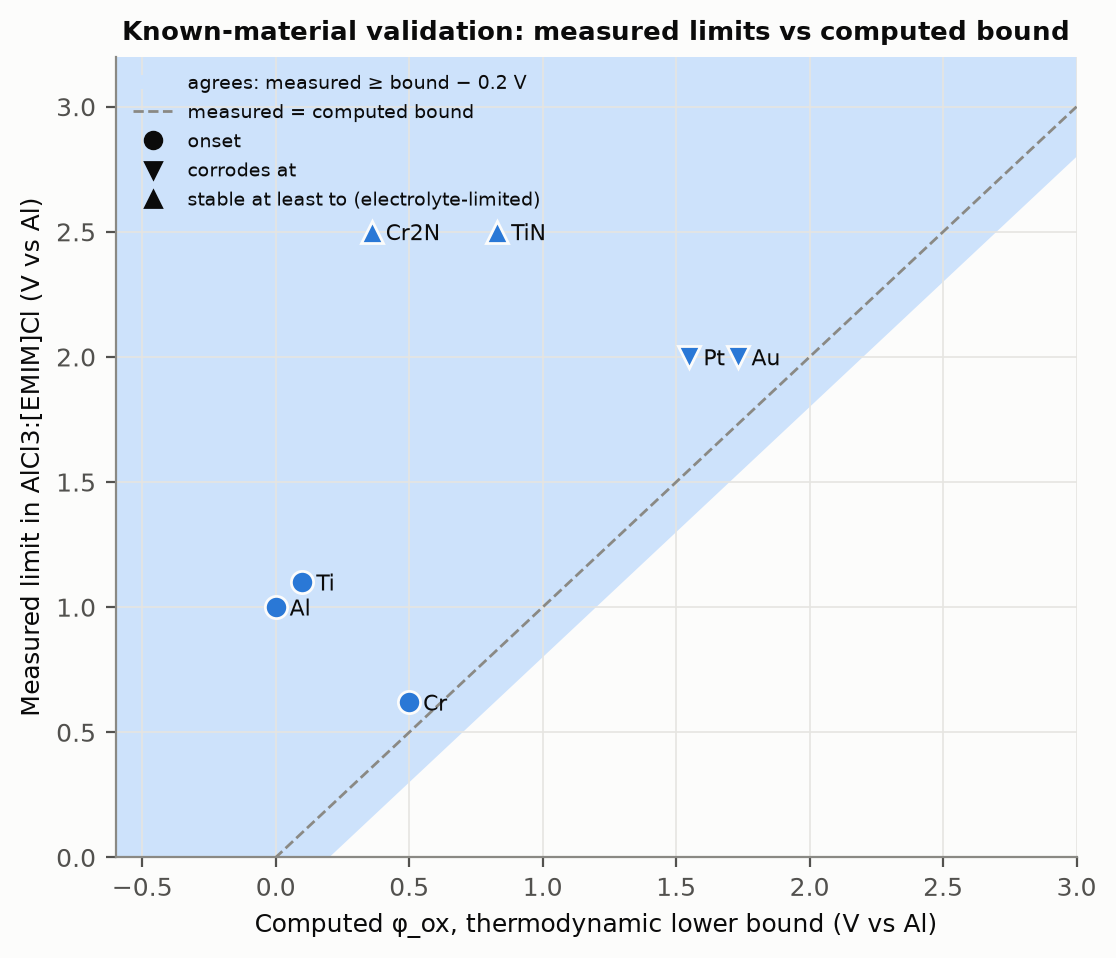
\includegraphics[width=0.62\textwidth]{10_validation.png}
\caption{Measured limits against the computed thermodynamic lower bound. The shaded region is ``agrees''.}
\label{fig:val}
\end{figure}

\noindent No material corrodes below its computed bound. The rank correlation between measured and computed onsets is $\rho = 0.74$ for $n = 4$ (Cr, Ti, Au, Pt), which indicates consistency, not statistical significance. The framework \textbf{cannot recognise kinetically protected materials}: TiN and \ce{Cr2N}, the best measured positive collectors, survive 1.7--2.1\,V beyond their thermodynamic bound. As a result the established collectors W, Mo and TiN all rank low in the screen, which identifies passivation and dissolution kinetics as the missing physics. In addition, filter F1 \textbf{wrongly rejects} \ce{Cr2N}: it is ICSD-known and measured stable, yet MP places it 245\,meV/atom above the hull. The threshold was not changed after this was found.

\subsection{Stability windows and ranking}
Figure~\ref{fig:win} shows the computed window of each high-priority candidate and literature reference, and Figure~\ref{fig:pareto} places all candidates on the two main ranking objectives.

\begin{figure}[H]
\centering
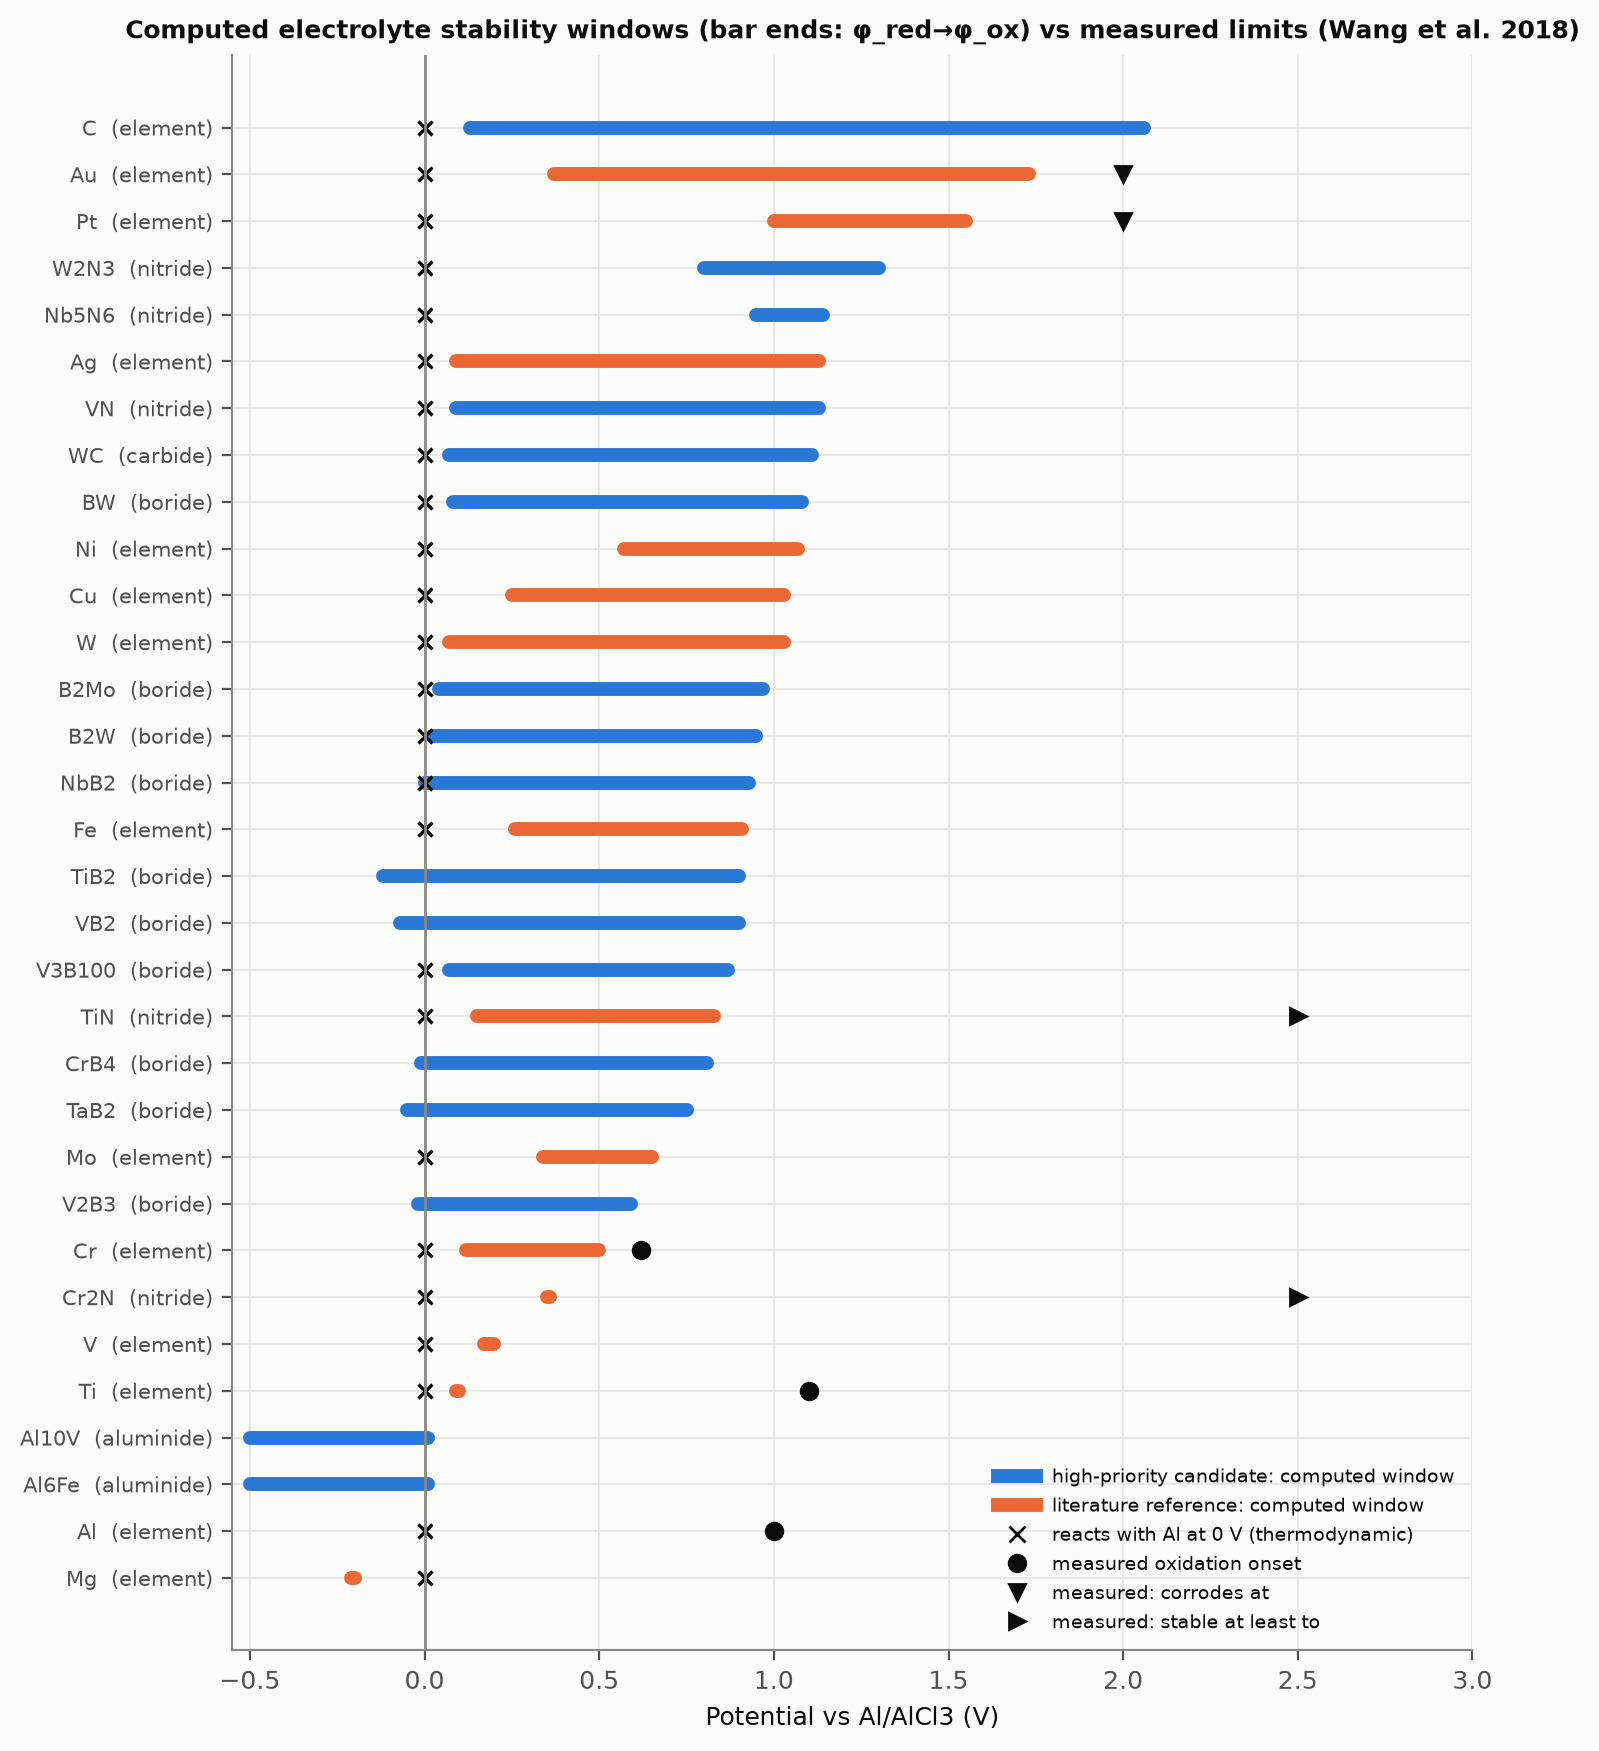
\includegraphics[width=0.66\textwidth]{08_stability_windows.png}
\caption{Computed stability windows ($\phired \rightarrow \phiox$) for high-priority candidates and literature references, with measured limits.}
\label{fig:win}
\end{figure}

\begin{figure}[H]
\centering
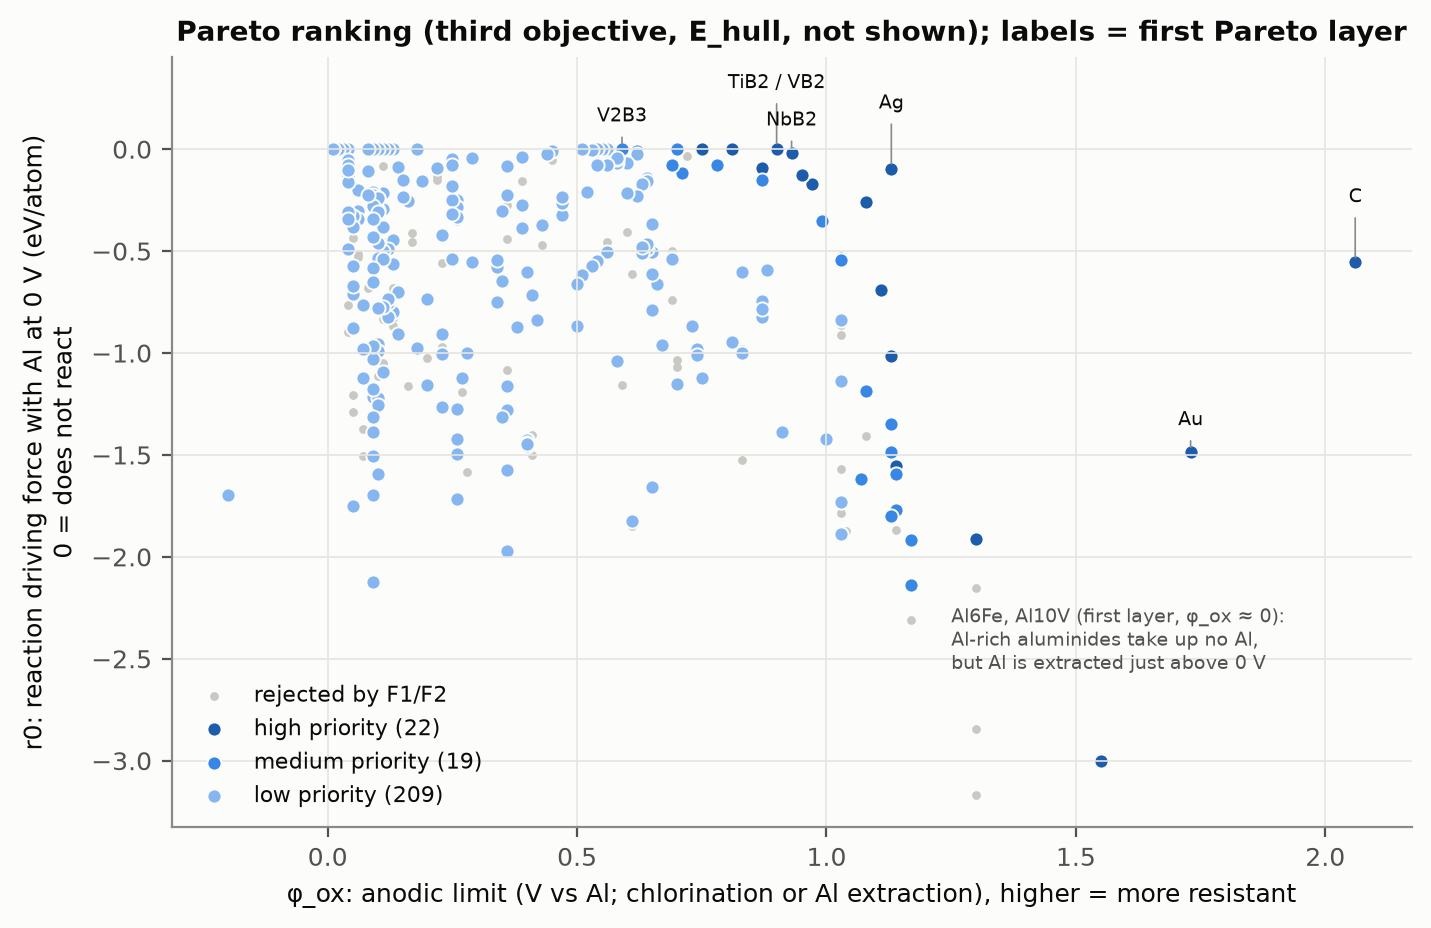
\includegraphics[width=0.85\textwidth]{09_pareto.png}
\caption{Pareto ranking: anodic limit against reactivity with Al at 0\,V, coloured by tier. The legend counts all 22 high-priority compositions, including the four Al-rich aluminides at $\phiox \approx 0$ discussed below; Table~\ref{tab:short} reports the remaining 18.}
\label{fig:pareto}
\end{figure}

The ranking places \textbf{22} compositions in the high-priority tier (Pareto layers 1--2). A Pareto front always contains the extreme point of each single objective, and four Al-rich aluminides (\ce{Al6Fe}, \ce{Al10V}, \ce{Al9Fe2}, \ce{Al23V4}) reach layer~1 on that technicality alone: they cannot take up more Al, so $r_0 = 0$, but Al is extracted from them as soon as the potential rises ($\phiox = 0.01$\,V). We therefore report the \textbf{18} high-priority compositions that also clear the lowest registered anodic scenario, $\phiox \ge 0.5$\,V. This is a reporting choice made after seeing the results, and it is the only one in this report; no threshold, filter or tier was changed. Wherever a count of 22 appears (Figures~\ref{fig:funnel} and~\ref{fig:pareto}), it is the full tier; wherever 18 appears, it is this shortlist.

\subsection{Preliminary shortlist}
Table~\ref{tab:short} lists the 18 high-priority candidates for future validation, that is, the high-priority tier restricted to $\phiox \ge 0.5$\,V. The complete list, with reasons, the 19 medium-priority candidates and 13 rejected examples, is in \texttt{results/shortlist.csv}.

\begin{table}[H]
\centering
\caption{The 18 high-priority candidates for future validation: the high-priority tier restricted to $\phiox \ge 0.5$\,V. $\phiox$ is given for the primary / alternative MP energy route. ``Inert'' means $|r_0| < 1$\,meV/atom as defined in Section~\ref{sec:window}; otherwise $r_0$ is the reaction energy with Al at 0\,V and the products are named. Values are computed (A); tier and confidence are inferred (C).}
\label{tab:short}
\small
\begin{tabular}{@{}llccrll@{}}
\toprule
Material & Family & $\phiox$ (V) & $\Ehull$ & $r_0$ & Products with Al at 0\,V & Confidence\\
 & & prim. / alt. & (meV/at.) & (eV/at.) & & \\
\midrule
C (graphite) & element & 2.06 / 1.82 & 3 & $-0.56$ & \ce{Al4C3} & higher\\
Au & element & 1.73 / 1.58 & 0 & $-1.49$ & \ce{Al2Au} & higher\\
Pt & element & 1.55 / 1.45 & 0 & $-3.00$ & \ce{Al21Pt8} & higher\\
\ce{W2N3} & nitride & 1.30 / 1.22 & 0 & $-1.91$ & \ce{Al5W} + \ce{AlN} & medium\\
\ce{Nb5N6} & nitride & 1.14 / 0.87 & 0 & $-1.55$ & \ce{AlN} + \ce{NbAl3} & lower\\
Ag & element & 1.13 / 1.17 & 0 & $-0.10$ & \ce{AlAg3} & higher\\
VN & nitride & 1.13 / 1.26 & 0 & $-1.02$ & \ce{Al3V} + \ce{AlN} & medium\\
WC & carbide & 1.11 / 0.99 & 0 & $-0.69$ & \ce{Al4C3} + \ce{Al5W} & lower\\
WB & boride & 1.08 / 0.94 & 0 & $-0.26$ & \ce{Al23B50} + \ce{Al5W} & higher\\
\ce{MoB2} & boride & 0.97 / 0.81 & 0 & $-0.17$ & \ce{Al23B50} + \ce{Al5Mo} & lower\\
\ce{WB2} & boride & 0.95 / 0.80 & 0 & $-0.13$ & \ce{Al23B50} + \ce{Al5W} & lower\\
\ce{NbB2} & boride & 0.93 / 0.82 & 0 & $-0.02$ & \ce{Al23B50} + \ce{NbAl3} & lower\\
\ce{TiB2} & boride & 0.90 / 0.77 & 0 & $0$ & \textbf{inert} & lower\\
\ce{VB2} & boride & 0.90 / 0.85 & 0 & $0$ & \textbf{inert} & higher\\
\ce{V3B100}\footnotemark & boride & 0.87 / 0.71 & 33 & $-0.09$ & \ce{Al23B50} + \ce{VB2} & lower\\
\ce{CrB4} & boride & 0.81 / 0.76 & 0 & $0$ & \textbf{inert} & lower\\
\ce{TaB2} & boride & 0.75 / 0.75 & 0 & $0$ & \textbf{inert} & higher\\
\ce{V2B3} & boride & 0.59 / 0.85 & 0 & $0$ & \textbf{inert} & higher\\
\bottomrule
\end{tabular}
\end{table}
\footnotetext{\ce{V3B100} (mp-1216517, space group $P222$) is boron with 2.9\,at.\% vanadium, is hypothetical in MP (no ICSD record) and is the only entry of its composition. It is most likely a dilute-substitution supercell rather than a distinct boride phase, so it should not be treated as a real candidate until its structure has been checked. It is left in the table rather than removed silently, because the ranking was not altered after the results were seen.}

\noindent\textbf{Rejected examples.}
\begin{itemize}[leftmargin=*,itemsep=1pt]
\item Not metallic (F2): \ce{Zr3N4}, \ce{Hf3N4}, \ce{Nb3N5}.
\item Outside the metastability window (F1): \ce{CrB2}, \ce{Cr2B}, CrSi, \ce{W9C4}, CrC, \ce{Al8Cr5}.
\item Al extracted at 0.01\,V: \ce{Al6Fe}, \ce{Al10V}.
\item Chlorinated at 0.10\,V: Ti.
\item Mg has no stability window at any potential: it is displaced by Al.
\end{itemize}

\subsection{Discussion}
Two groups of candidates emerge, for different reasons. (i) \emph{High anodic limit}: graphite, Au, Pt, the W, Nb and V nitrides, WC and the W borides. These are thermodynamically safe up to about 1--2\,V after complete stripping, but can alloy with, or be reduced by, Al at the plating potential. (ii) \emph{Inert to Al at 0\,V}: \ce{TiB2}, \ce{VB2}, \ce{CrB4}, \ce{TaB2} and \ce{V2B3}. These are the only metallic, stable compounds that cannot react with deposited Al while also having anodic limits of 0.6--0.9\,V, which is adequate if the negative collector is not driven above about 0.6\,V. Across all three tiers, only 11 of the 250 metallic, stable compositions are both inert to Al ($|r_0| < 1$\,meV/atom) and anodically stable to at least 0.5\,V: nine transition-metal borides (\ce{TiB2}, \ce{VB2}, \ce{CrB4}, \ce{TaB2}, \ce{V2B3}, \ce{Ta3B4}, \ce{V3B4}, \ce{ZrB2}, \ce{HfB2}) and two disilicides (\ce{CrSi2}, \ce{TaSi2}). Five of those borides reach the high-priority tier and appear in Table~\ref{tab:short}; the others sit in the medium and low tiers because their anodic limits are lower. The borides in Table~\ref{tab:short} that are \emph{not} inert (WB, \ce{MoB2}, \ce{WB2}, \ce{NbB2}) still react only weakly with Al, by $0.02$--$0.26$\,eV/atom, against $1.0$--$3.0$\,eV/atom for the metals and nitrides above them. Borides therefore populate both groups, which makes them the most consistent family in the screen. We found no chloroaluminate experiment on them, so they are the clearest testable prediction of this work.

\paragraph{Cost is not a screening objective.} Au and Pt rank high on thermodynamics alone, but a technology whose appeal is low-cost stationary storage will not use them. They are best read as references that mark the top of the achievable anodic range, alongside graphite, which is both cheap and the most stable material in the screen. The practically relevant group is the transition-metal borides. Cost, abundance and processability are not descriptors in this framework, and adding them is a candidate for the next stage.

The validation also shows what the framework cannot yet do. Its central descriptor guarantees stability but does not predict it: well-performing positive collectors such as TiN owe their stability to kinetics or surface films. The ranking should therefore be read as ``thermodynamically safe'' rather than ``best'', and materials known to passivate need a separate, kinetic descriptor.

\subsection{Limitations}
\begin{enumerate}[leftmargin=*,itemsep=2pt]
\item \textbf{Bulk thermodynamics only.} $\phiox$ is a lower bound; passivation and kinetics are outside the model, so kinetically protected materials are under-rated.
\item \textbf{No surface physics yet.} Al nucleation affinity (adsorption or binding energy, interfacial energy, lattice mismatch) is not available in the current dataset and is proposed for Phase~2 (DFT). MP work functions and surface energies exist for only 18 of 330 compositions (elements).
\item \textbf{Idealised electrolyte.} \ce{AlCl3} is taken at unit activity, chloride products are not dissolved or complexed, and there is no organic cation; the energies are at 0\,K.
\item \textbf{DFT error.} The two MP energy-mixing routes differ by up to 0.42\,V in $\phiox$; \ce{Cr2N} is misplaced by F1. MP provides no per-entry uncertainty for mixed entries.
\item \textbf{Conduction proxy.} Metallic in PBE is not the same as conductive, and native oxides are ignored.
\item \textbf{Sparse literature.} Only four numeric onsets, all from one paper, and mostly from positive-electrode tests; per-material anode-free data were not accessible.
\item \textbf{ML uncertainty.} None of the tested proxies tracks the error.
\item \textbf{Target truncation.} The $\Ehull \le 1$\,eV/atom cut-off truncates the target range of elemental entries, so the $R^2$ values here are not comparable with an unfiltered study.
\end{enumerate}

\noindent\textbf{Claims not made.} No substrate has been ``discovered''; ML does not predict battery performance; no nucleation, adsorption or corrosion-rate values are reported; four literature points support consistency, not significance; and the computed potentials are thermodynamic bounds, not predicted measured onsets.

% =====================================================================
\pagebreak
\section{Conclusions}
\begin{itemize}[leftmargin=*,itemsep=2pt]
\item A reproducible screening framework on real Materials Project data is in place. Its thresholds and validation rules were fixed before any result was seen, and every output is labelled as computed, literature or inferred.
\item The stability-window descriptor behaves as a thermodynamic lower bound: it shows no contradiction with the verified literature, but it cannot see kinetic protection.
\item No stable metallic composition is both anodically stable to 1\,V and inert to Al at the plating potential. The Pareto ranking puts 22 compositions in the high-priority tier, of which 18 also clear the lowest anodic scenario and are reported as the shortlist; transition-metal borides are the most consistent family and the clearest prediction to test next.
\item Composition-only ML generalises to unseen chemical systems ($R^2 = 0.93$) but less to unseen elements ($R^2 = 0.63$), and its uncertainty estimates do not yet work.
\end{itemize}

% =====================================================================

% =====================================================================
\pagebreak
\section{Future work}
\label{sec:plan}

The validation in Section~\ref{sec:val} points to what is missing, so the next steps follow from it rather than from a wish list. They are given in the order I intend to attempt them, not as a guarantee of completion: the surface work in particular depends on DFT software and HPC time that I still have to arrange, and if that access does not come through in time, the kinetic and electrolyte descriptors below can be developed from Materials Project data alone.

\begin{enumerate}[leftmargin=*,itemsep=3pt]
\item \textbf{Surface energetics of the boride candidates (first priority).} Slab models of \ce{TiB2}, \ce{VB2} and \ce{CrB4}, with W, TiN and graphite as references, to obtain the Al adsorption energy and the Al/substrate interfacial energy, plus the lattice mismatch with Al(111). This is the descriptor the present framework lacks, and it is what decides nucleation. Subject to arranging DFT and HPC access.
\item \textbf{A kinetic or passivation descriptor.} The clearest gap the validation exposed: TiN and \ce{Cr2N} survive far beyond their thermodynamic bound. I plan to test whether the solubility of the chloride products, or the formation of a surface film, separates the materials that passivate from those that dissolve.
\item \textbf{A more realistic electrolyte.} An \ce{AlCl3} activity correction for acidic melts, and complexed chloride products, to test how far the 0.2\,V tolerance used in validation actually stretches.
\item \textbf{Completing the literature benchmark.} Obtaining the per-material results of~\citep{WangL2021} and~\citep{Shi2019} would let the Cu, Ag, Mg and graphite-paper rows be scored instead of left unverified.
\item \textbf{Calibrated ML uncertainty.} Conformal intervals fitted on the grouped folds, tested the same way as in Section~\ref{sec:mlres}. Only if that works does screening hypothetical ternary borides and nitrides become defensible.
\item \textbf{A combined ranking, and experiment if a collaboration can be arranged.} Bulk, surface and kinetic descriptors together, compared against whatever experimental data become available; the measurement I would most like is a CV and an Al plating/stripping efficiency for sputtered \ce{TiB2} or \ce{VB2} against TiN and W.
\end{enumerate}

\noindent The end-semester report and presentation are due on 24 and 27 November respectively.

% =====================================================================

\bibliography{./bibliography.bib}

% =====================================================================
\appendix
\pagebreak
\section{Additional figures}

\begin{figure}[H]
\centering
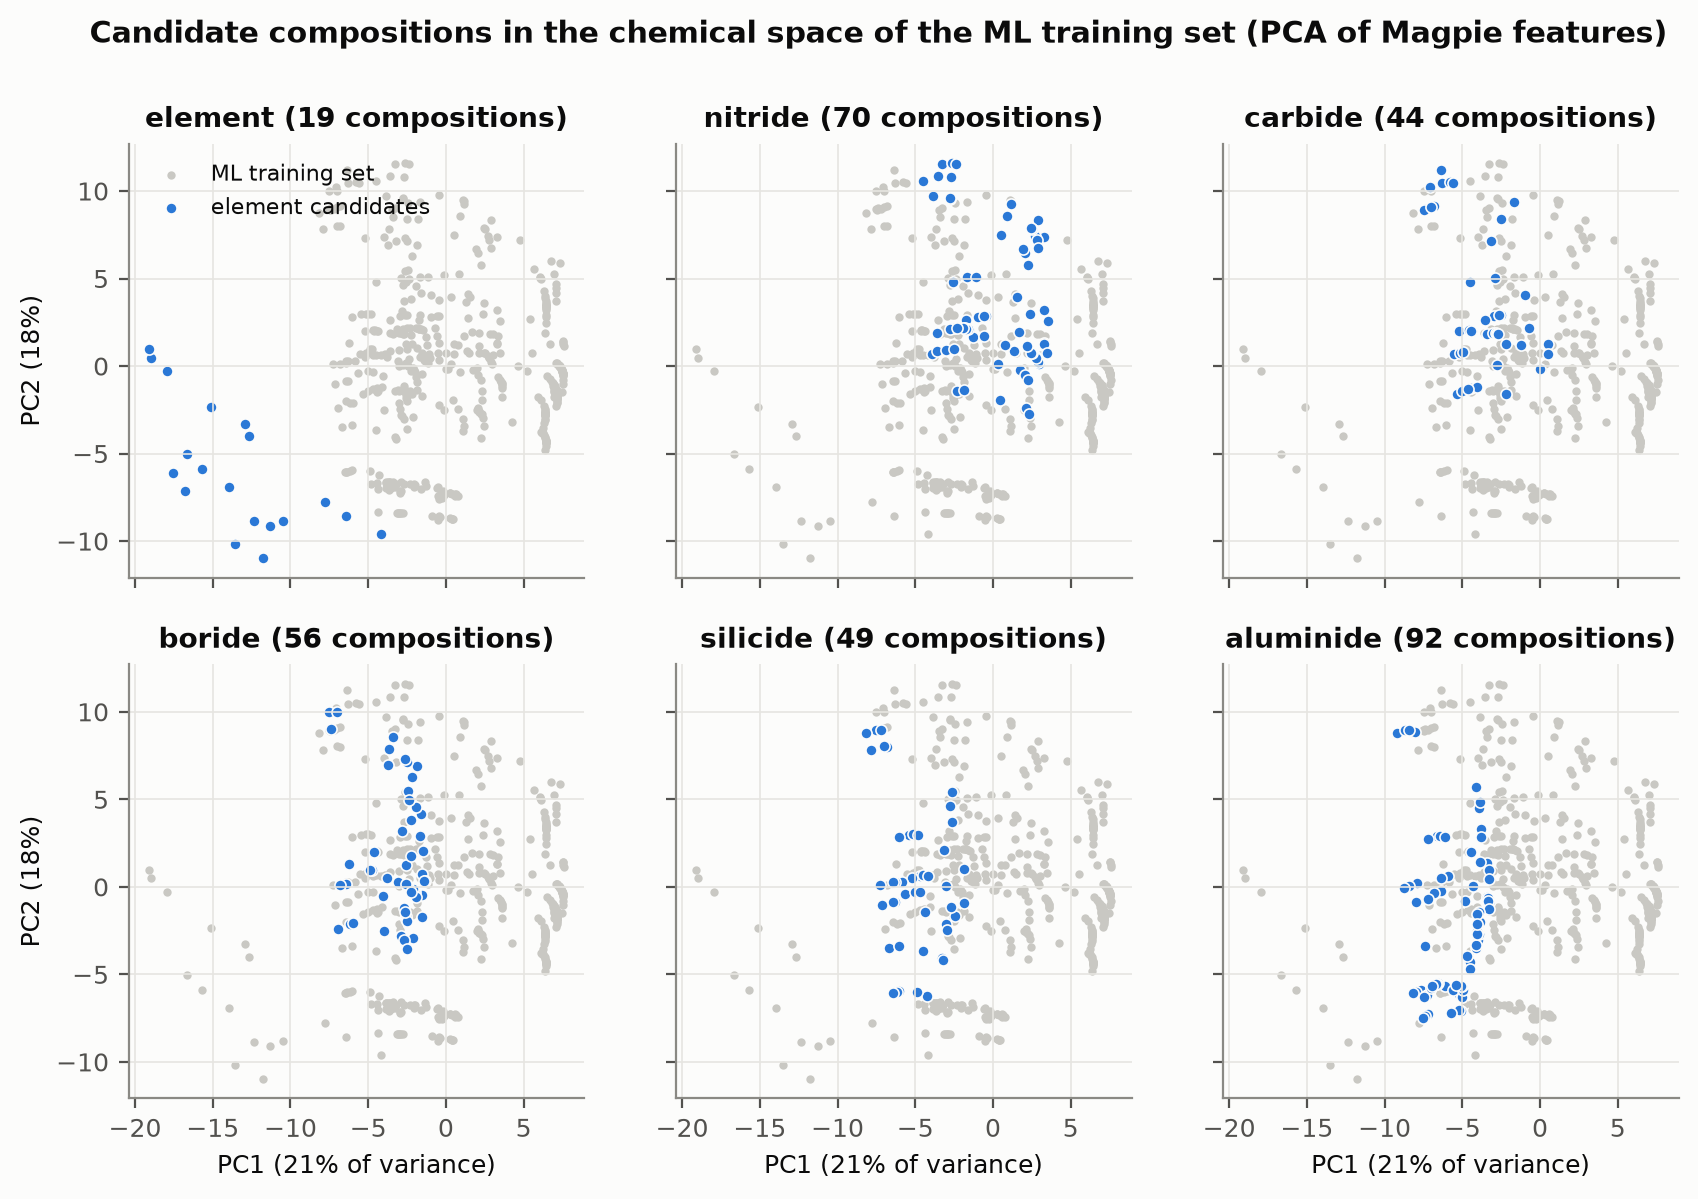
\includegraphics[width=0.95\textwidth]{01_chemical_space.png}
\caption{Screening families in the composition space of the ML training set (PCA of Magpie features).}
\end{figure}

\begin{figure}[H]
\centering
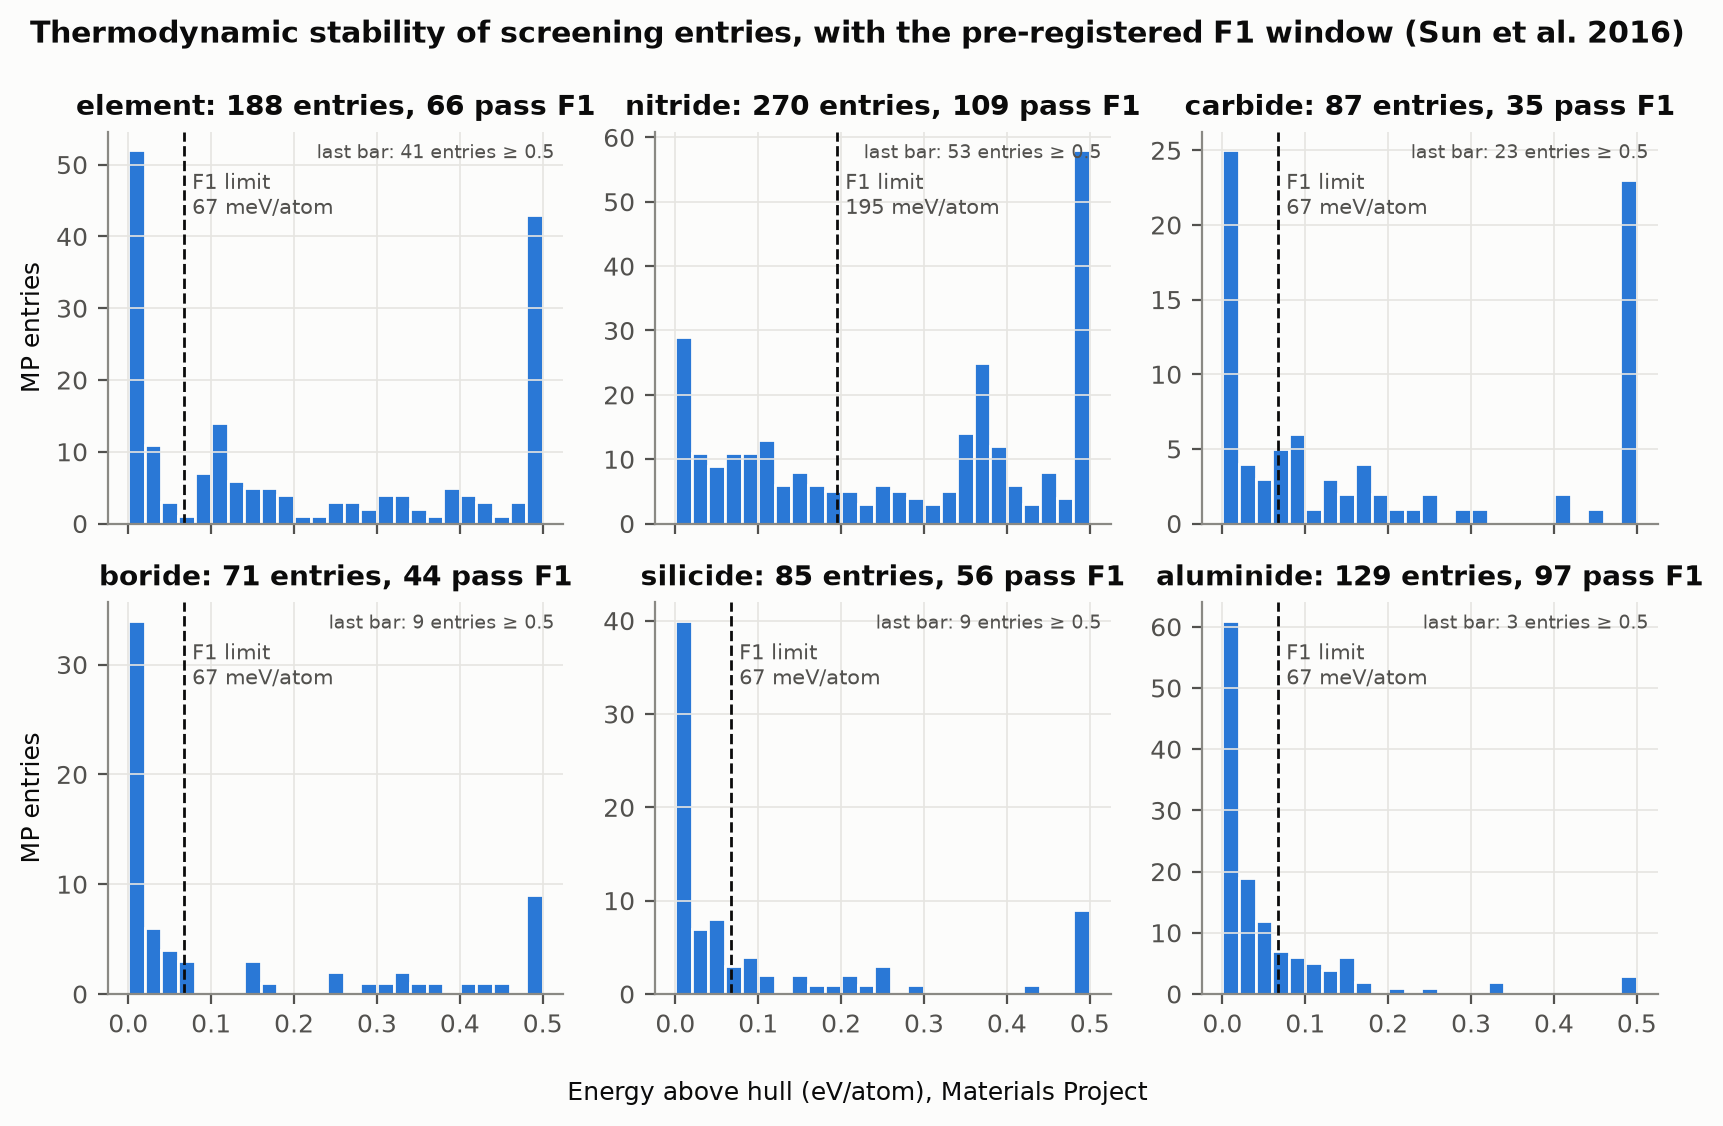
\includegraphics[width=0.95\textwidth]{02_stability_distributions.png}
\caption{Energy above hull of screening entries by family, with the F1 window~\citep{Sun2016}.}
\end{figure}

\end{document}
